\documentclass[PWPL]{article}
\usepackage{PWPL}
\usepackage{tipa}
\usepackage{enumerate}
\usepackage{graphicx}
\usepackage{multirow}
\usepackage{amsmath}
\usepackage{caption}
\usepackage{subfigure}
\title{The Social Perception of a Sound Change in York, Northern England}
\author{Daniel Lawrence}
\begin{document}
\maketitle
%\abstract{A core claim of sociolinguistic theory is that language variation functions as a social-semiotic resource, providing an explanation for patterns of group-level convergence and divergence with regard to ongoing linguistic change. What is lacking from existing work is a framework for formulating testable hypotheses regarding the relationship between listeners’ social perceptions of innovations and their productive behavior with regard to those innovations. With a view to addressing this problem, this paper presents an account of the fronting and diphthongization of the tense back vowels /u/ and /o/ in York, Northern England. After presenting evidence of ongoing change in these vowels, the paper evaluates a recent account of the role of social indexicality in constraining the changes through a novel experimental paradigm. The findings contradict previous accounts of change in this community -- for example, despite its rapid and uniform incrementation and apparent lack of class-stratification in production, /u/-fronting emerges as a robust cue to socioeconomic status in perception. While the absence of fronted /o/ monophthongs in the speech of younger speakers has previously been interpreted as evidence of their stigmatization, there is no support for this in the perception data. Intriguingly, there is evidence of structured variability in listeners’ social-perceptual responses -- the social groups who lead the changes in production appear to be more sensitive to their social-indexical significance in perception.}

\section{Introduction}

A core finding of sociolinguistics is that sound changes may become available as a social-semiotic resource as they propagate through a speech community. The social evaluations attached to linguistic innovations are often used as an explanation for differences in the trajectories of parallel changes (e.g. Labov et al. 2014), or to explain differences in the rates of adoption of innovations across social groups (e.g. Hall-Lew, 2009). While much work has framed these evaluations by referring to their \textit{salience} or the degree of \textit{stigma} attached to them, recent studies have attempted to develop a more sophisticated understanding of the types of social meaning communities may attach to variation. In particular, the notion of the \textit{persona} has risen to prominence -- it is argued that speaker-listeners' social perceptions of linguistic variation tend to be structured around locally-relevant stereotypical figures such as the `valley girl' or `burnout' (Eckert, 2008; Moore \& Podesva, 2009; D'onofrio, 2015). Applying this perspective to sound change, it has been argued that innovations which come about due to global processes of change (such as chain-shifting principles) may become attached to local stereotypes in certain speech communities, resulting in divergent behavior on the part of some groups of speakers. 

While this approach provides an intuitive account of how global processes of change might interact with local social-semiotic systems in influencing the speech patterns of a given community, it raises the issue of how the social meanings proposed can be verified, and how their role in constraining the change under study can be diagnosed. This paper approaches this problem by combining the acoustic analysis of a sound change in progress with the results of an innovative social perception experiment which tested listeners' social intuitions regarding phonetic variation in the changing forms. This strategy enables the quantification of the degree to which listeners associate different speech forms with different social stereotypes, allowing quantitative predictions to be formed regarding which forms are associated with which social meanings, and for which groups of speaker-listeners. 




%\subsection{Sampling}

%Data are taken from a corpus of recordings collected from a convenience sample of 52 York residents born between 1935 and 2000. All participants were born and raised in York, and had at least one parent from York.Table 1 provides the basic demographic information of the sample, including participants' gender and year of birth (collected from a post-interview questionnaire), and their grouping according to a \textit{mobility index}. This index was one of three factors derived from informants' responses to the interview questions (see section x.x).

%\vspace*{6pt}
%\begin{table}[ht]
%\small
%\centering
%\begin{tabular}{l|l|l|l|l}
%Mobility index&\multicolumn{2}{l|}{Upper}&\multicolumn{2}{l}{Lower}\\
%\hline
%Gender& Female& Male & Female & Male\\
%\hline
%1935-1960 & 6&5&2&2\\
% 1961-1980& 2 &4&4&0\\
%1981-2000&  8&11&3&5\\

%\end{tabular}
%\caption{Characteristics of the speaker sample}
%\end{table}
%\vspace*{6pt}

%\subsection{Social coding}

%In addition to collecting each speaker's year of birth and gender, three social indices were created based on a set of questions asked during the sociolinguistic interview. Three underlying dimensions were derived from an exploratory factor analysis of these responses -- a general SES index, a local identity index, and a mobility index; for brevity, the specific details of this factor analysis will be left for a future version of this work. The general SES index groups together a measure of the speaker's level of education and employment status. The local identity index measures the degree to which each individual identifies as someone from York, and the extent to which they are invested in the local community. The mobility index groups together a set of characteristics related to geographical and social mobility, e.g. whether or not the speaker travels regularly within the UK; whether or not they have worked and studied in York for an extended period, and whether or not they plan to stay in York permanently.

%\subsection{Production data}

%The data include a) a 100-item wordlist, including 15 tokens of each vowel in a range of phonetic environments plus fillers; b) a map task (Anderson et al., 1991) using a selection of words from the word list and c) a sociolinguistic interview, including a range of questions relevant to the speakers' social background and identity with regard to York and the north of England. 

%Vowels were segmented from the first to the last glottal pulse visible in the spectrogram, and measurements of F1, F2 and F3 were taken at 20 equidistant points along the vowel trajectory. The present analysis will focus on F2 trajectories, which provide a relatively reliable reflection of the degree of fronting and diphthongization for these vowels. Measurements were normalized using the centroid method of Watt \& Fabricius (2002), using the mean midpoint values of each speakers' \textipa{/A/} and \textipa{/i/} productions as reference values. The formant values provided in the present analyses are of the form $F^n/S (F^n)$, i.e. the ratio of the measured frequency in Hz to the centroid frequency of that formant for the speaker being analyzed.


\section{/u/ and /o/ fronting in York}
The data for the present study are taken from a corpus of recordings collected from a convenience sample of 52 York residents born between 1935 and 2000. F1 and F2 measurements were taken at 20 equidistant points along the vowel trajectory, and these values were normalized using the normalization method of Watt \& Fabricius (2002). Figures 1(a) and 1(b) plot these measurements as a function of speaker year of birth. Both vowels show evidence of fronting, with the most rapid and incremental fronting affecting /u/. The fronting of /o/ appears to be less regular, in the sense that speakers are less tightly clustered around the regression line in 1(b) than 1(a).
\begin{figure}[!ht]
\centering
\caption{Variation and change in /o/ and /u/}
\subfigure[]{
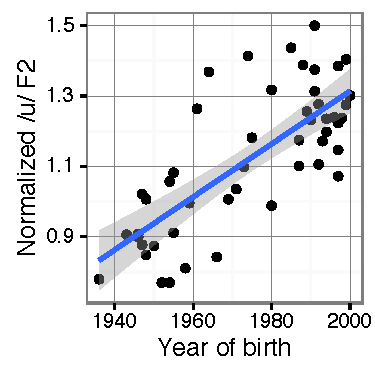
\includegraphics[scale=0.7]{uw_yob_small.pdf}}
\subfigure[]{
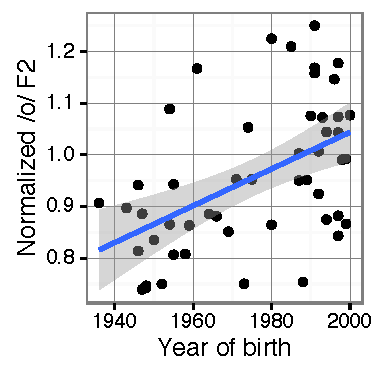
\includegraphics[scale=0.7]{ow_yob_small.pdf}}
\subfigure[]{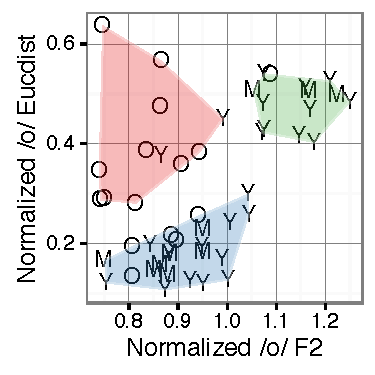
\includegraphics[scale=0.7]{ow_front_dip_small.pdf}}
%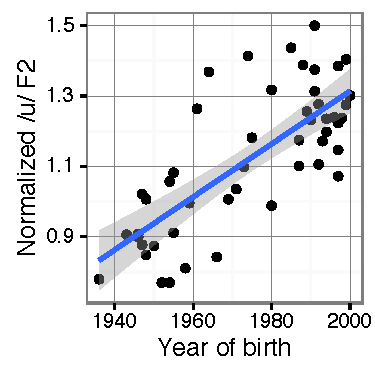
\includegraphics[scale=0.7]{uw_yob_small.pdf}
%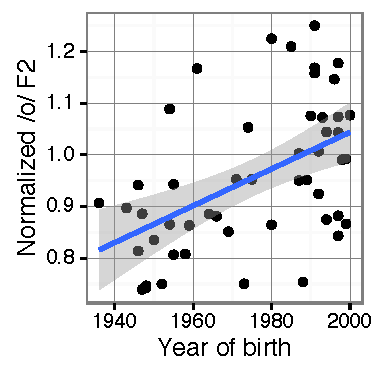
\includegraphics[scale=0.7]{ow_yob_small.pdf}
\end{figure}

Plotting Euclidean distance and F2 values in two-dimensional space demonstrate how change in /o/ involves both fronting and diphthongization. This is demonstrated in Figure 1(c)
The colored hulls show the output of a density-based clustering algorithm on these data, which identifies three groups of speakers -- those with back /o/ realizations and middle/high Euclidean distances; those with back /o/ realizations and low Euclidean distances, and those with fronted /o/ realizations and high Euclidean distances. It should also be noted that membership of each cluster is predictive of the age of the speaker --  back, diphthongal speakers are most likely to be in the oldest age group; back, monophthongal speakers are most likely to be in the middle or youngest age group, and speakers who produce front diphthongs are most likely to be in the youngest age group. The pattern appears to involve a reduction of the range of variation in diphthongization of back /o/ variants, and the adoption of very fronted, diphthongal variants among a subgroup of younger speakers. 

In summary, the production data provide evidence for the fronting of /u/ and /o/ in this community. While /u/ fronting appears to proceed in a relatively uniform manner, /o/ fronting appears to have taken place more slowly and spread less uniformly across the population. Considering the role of /o/ diphthongization in this process reveals that /o/ fronting is restricted to speakers with diphthongal /o/ -- while the fronting of monophthongal /o/ is in principle possible, and even attested in other Northern British varieties of English (Watt \& Tillotson, 2001), there appears to be an absence of fronted, monophthongal speakers in this sample, evident in the lack of datapoints in the bottom right-hand quadrant of 1(c).

%A schematization of the trajectory of change in /u/ and /o/ is provided below. The oldest speakers in the sample produce relatively back /u/ and /o/ variants, and exhibit variation in terms of /o/ diphthongization (i). The apparent conditional relationship between /u/ and /o/ fronting implies that change in /u/ actuated before that in /o/, allowing an intermediate state to be posited (ii). At this stage, the centralization of /u/ had begun, but /o/ remained relatively back. The present stage of the change (iii) involves further fronting of /u/, and the sharp separation of speakers into two groups with regard to their /o/ production -- those with very front diphthongs, and those with comparatively back monophthongs. 


%\begin{table}[ht]
%\centering
%\setlength{\tabcolsep}{0.5cm}
%\label{haddican-results}
%\begin{tabular}{llllllllll}
%&i.&ii.&iii.&\\
%/o/ &    o $\sim$ \textipa{oU} &  o $\sim$ \textipa{oU}        &  o       &  \textipa{\textschwa y}                                  && \\
%/u/ &  \textipa{u} &  \textipa{0} &  \textipa{y} & \textipa{y}                    &           &                  &\\
%&   &   &  &                    &           &                  &\\
%\end{tabular}
%\end{table}

These data are generally consistent with Haddican et al.`s (2013) recent findings on /u/ and /o/ fronting in York. The patterning of these changes raises two key questions:

\begin{enumerate}[i)]
\item{What causes /u/ to front so rapidly and uniformly in comparison to /o/?}
\item{Why do younger speakers avoid fronting monophthongal /o/?}
\end{enumerate}

While a number of social, cognitive and linguistic factors might be invoked to explain these patterns, the remainder of this paper will focus on the proposal of Haddican et al. (2013), whose explanation centers around the social indexicality of variation in the changing vowels.  With regard to the relative uniformity of change in /u/ vis-a-vis /o/, the authors propose that the fronting of /u/ is less important as a social-indexical resource to York speakers in comparison to the fronting and diphthongization of /o/. Under this account, this relative lack of social indexing allows /u/ fronting to propagate rapidly and relatively uniformly across the community, since the adoption of fronted /u/ variants will have limited social consequence for speakers. In contrast, /o/ diphthongization is claimed to be strongly associated with socioeconomic status and `local' regional identity. Such claims are reasonable, since the diphthongization of the mid vowels is known to be a shibboleth of Northern/Southern English identity, at least in production (Watt, 2000; Beal, 2004). The implication of Haddican et al.'s (2013) proposal is that change in /o/ might be slower and less uniform than change in /u/ due to the participation of /o/ in a pattern of social indexing. 

The author's third key claim is that fronted, monophthongal /o/ is associated with a stigmatized working-class stereotype, the `chav'. This stereotype, reflecting an individual who is typically unemployed and engages in antisocial behaviour, has become a key feature of popular discourses around social class in the United Kingdom (see e.g. Hayward \& Yar, 2006). Haddican et al. (2013) provide convincing evidence from ethnographic interviews that this social category is important to younger York residents, and propose that the absence of fronted, monophthongal /o/ in their data may be explained by younger speakers' avoidance of forms enregistered as `chav' speech. 

Haddican et al.`s (2013) social-indexical account of variation and change in /o/ and /u/ represents a common pattern of argument in sociolinguistic work -- inferring a social signalling system based on observed production patterns. While their explanation is intuitive, and convincingly supported by their ethnographic data, it should be recognised that it represents one possibility in a potentially very large explanation space. In order to evaluate this proposal, the present work attempts to formulate and test a set of concrete predictions regarding the social perception of variation in the target vowels. One way of thinking about any claim regarding the social meaning of phonetic variation is to express it as model of social categories distributed in multidimensional phonetic space. These social categories may include `macro-level' meanings such as \textsc{local} or \textsc{working class}, or more locally-specific personae such as \textsc{chav}. An example for /u/ and /o/ variation in York, based on Haddican et al. (2013), is provided in Figure 2, which represents the categories \textsc{local} \textsc{working class} and \textsc{chav} in F2-Euclidean distance space.

\begin{figure}[ht]
\centering
\caption{Hypothesised mappings of indexical meanings to F2-Euclidean distance space}

\includegraphics[scale=0.2]{u_hypothesis_space.png}
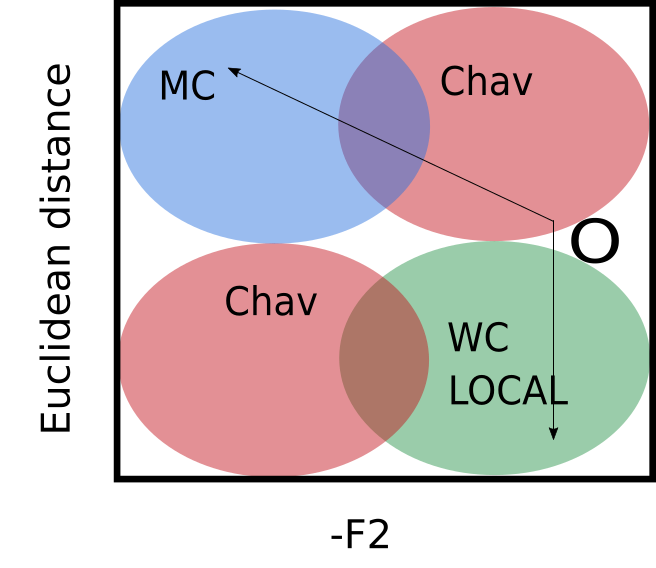
\includegraphics[scale=0.2]{o_hypothesis_space.png}
\end{figure}

Figure 2 includes an addition to the argument presented in Haddican et al. (2013), with the inclusion of the hypothesis that back /o/ monophthongs are also enregistered as part of the \textsc{chav} persona. Since back /o/ diphthongs as well as fronted /o/ monophthongs are absent from the speech of younger speakers, it is reasonable to extend Haddican et al.`s (2013) proposal to include these forms. 

Understanding a claim regarding social indexicality in the manner shown in Figure 2 allows concrete predictions regarding the social perception of the linguistic variables under study. For example, when a listener hears a talker use a back, diphthongal variant of /o/, we predict that they are most likely to assign that talker to the \textsc{chav} category. With increasing fronting, we predict that they will be increasingly more likely to assign \textsc{middle class} to that talker. This pattern of reasoning can be extended across all combinations of phonetic parameters and social categories (see section x.x)

In order to test these predictions, a social perception experiment was conducted with the same speaker sample described in section x.x. The aim of this experiment was to quantify the extent to which York listeners associate the proposed social categories with /u/ and /o/ variation. The design of this experiment is described in the following section.

\section{The social perception of \textipa{/u/} and \textipa{/o/} variation}

\subsection{Experimental design}
\subsubsection{Auditory stimuli}

The auditory stimuli consisted of resynthesized tokens of the words \textit{too}, \textit{food} (/u/), \textit{toast} and \textit{so} (/o/), read by a 24-year-old middle-class speaker from York. The stimuli were resynthesized using a \textit{Praat} script based on Alku et al.'s (1999) \textit{IAIF} method. The complete set of \textipa{/o/} stimuli included tokens representing three steps of fronting of monophthongal variants and three steps of two types of fronting (targeting the vowel onset and offglide) across diphthongal tokens. These included a back diphthongal realization, two steps of fronting at the vowel onset, and two steps of fronting of the offglide. The \textsc{/u/} stimuli included examples of three levels of fronting, from a back realization to very fronted, as well as three identical tokens with lowered onsets, resulting in more diphthongal tokens.

Figures 3.1-3.3 give the IPA symbols which will be used to refer to the tokens in the analyses. 

\begin{table}[ht]
\caption*{Figure 3.2: \textsc{goat} variants used in the experiment}
\centering
\scriptsize
\begin{tabular}{llllll}
&&&&&\\
                  &           & \textit{Fronting}          &             &                   &\\
                &  \multicolumn{3}{l}{$\xleftarrow{\hspace*{7.5cm}}$  }   &                              \\
\multirow{5}{*}{$\rotatebox[origin=c]{90}{$\underleftarrow{\rule{1cm}{0pt}Diphthongization}$}$}                 &&&& &                \\
               & \LARGE{\textbf{\textipa{\o:}}}&\LARGE{\textbf{\textipa{8:}}}&\LARGE{\textbf{\textipa{o:}}}&&\\
 & Mid-front monophthong & Mid-central monophthong  & Mid-back monophthong  &         &          \\
        &\LARGE{\textbf{\textipa{eU}}}&\LARGE{\textbf{\textipa{9U}}}&\LARGE{\textbf{\textipa{oU}}}&&\\
                   & Mid-front diphthong  & Mid-central diphthong & Mid-back diphthong\\
                   &(fronted onset)&(centralized onset)&&&\\
                   &\LARGE{\textbf{\textipa{9y}}}&\LARGE{\textbf{\textipa{90}}}&&&\\
                   &Mid-front diphthong &Mid-central diphthong &&&\\
                   &(fronted offglide)&(centralized offglide)&&&\\
\end{tabular}
\end{table}
\begin{table}[ht]
\caption*{Figure 3.3: \textsc{goose} variants used in the experiment}
\centering
\scriptsize
\begin{tabular}{llllll}
&&&&&\\
                  &           & \textit{Fronting}          &             &                   &\\
            &  \multicolumn{3}{l}{$\xleftarrow{\hspace*{5cm}}$  }  &                              \\ 
     \multirow{5}{*}{$\rotatebox[origin=c]{90}{$\underleftarrow{\mathsf{\textit{Diphthongization}}}$}$}        
                      
 &&&&       &\\
        &\LARGE{\textbf{\textipa{Yu}}}&\LARGE{\textbf{\textipa{0u}}}&\LARGE{\textbf{\textipa{Uu}}}&&\\
                   & High-front  & High-central& High-back\\
               & \LARGE{\textbf{\textipa{eu}}}&\LARGE{\textbf{\textipa{9u}}}&\LARGE{\textbf{\textipa{7u}}}&&\\
       & High-front  & High-central& High-back\\
 & (lowered onset)  & (lowered onset)  &(lowered onset) \\
\end{tabular} 
\end{table}

\subsubsection{Visual stimuli}

Visual stimuli consisted of eight images representing individuals of different ages (older vs younger), different occupations (working class vs middle class) and of different regional background (urban vs rural).  The social dimensions of older/younger, working-class/middle-class, and urban/rural were included based on the findings of a set of ethnographic interviews conducted prior to the main data collection phase, as well as the claims made by Haddican et al. (2013). Each stimulus image contained three components -- an image of a face (providing information about the character's age), an image of a place of work/study (providing information about the character's social status) and an image of an urban or rural location (providing information about the regional background of the character). The eight images represent all possible combinations of these three social dimensions, shown in Figure 3.7.

\begin{figure}[ht]
\caption{Visual stimuli}
\centering
\begin{tabular}{ccccc}
\multirow{2}{*}{$\rotatebox[origin=t]{90}{$\overbrace{\rule{0.5cm}{0pt}\mathsf{\textit{Rural}}\rule{0.5cm}{0pt}}$\hspace*{-2cm}}$} &
\includegraphics[scale=0.25]{M_O_MC_L_1.png} & 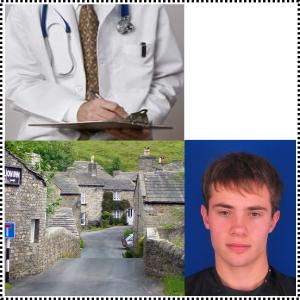
\includegraphics[scale=0.25]{M_Y_MC_L_1.png} 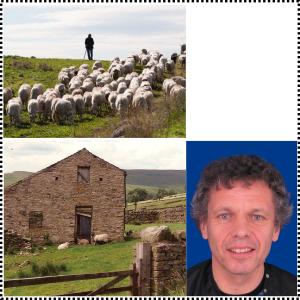
\includegraphics[scale=0.25]{M_O_WC_L_1.png} &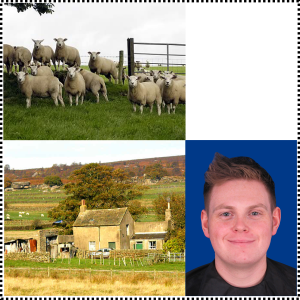
\includegraphics[scale=0.25]{M_Y_WC_L_1.png} \\ 
 $\rotatebox[origin=t]{90}{\hspace*{1.5cm}$\overbrace{\rule{0.5cm}{0pt}\mathsf{\textit{Urban}}\rule{0.5cm}{0pt}}$}$
    &
\includegraphics[scale=0.25]{M_O_MC_NL_1.png} & 
\includegraphics[scale=0.25]{M_Y_MC_NL_1.png} 
\includegraphics[scale=0.25]{M_O_WC_NL_1.png} & 
\includegraphics[scale=0.25]{M_Y_WC_NL_1.png}\\
\end{tabular}
\end{figure}
\vspace*{-2.25cm}
\begin{figure}[ht]
\centering
\begin{tabular}{lllll}


    &\multicolumn{4}{l}{
    $\underbrace{\rule{1cm}{0pt}{\textit{Age: Older/Younger}}\rule{1cm}{0pt}}$$\underbrace{\rule{1cm}{0pt}{\textit{Age: Older/Younger}}\rule{1cm}{0pt}}$}\\

    &\multicolumn{4}{l}{
$\underbrace{\rule{2.5cm}{0pt}{\textit{Social class: Middle/Working}}\rule{2.5cm}{0pt}}$}\\
   \end{tabular}
\end{figure}

The characters were designed to be feasible York personae, based on stereotypes discussed in the ethnographic interviews. Thus, the intersection of older, middle-class, and rural is represented by a doctor in a rural Yorkshire village (a), while the corresponding middle-class character is represented as a middle-aged businessman associated with a well-known insurance company (e). In all cases, the choice of component images reflects comments made by participants during the ethnographic interviews. A key claim made by Haddican et. al. (2013) is that fronted monophthongal \textsc{goat} variants are associated with a working-class youth stereotype called a `chav'. In this experiment, the `chav' is treated as the intersection of the urban, young and working-class dimensions, represented by the character in image (h). The non-facial images were taken from public domain collections, and the faces were selected from the Stirling ESRC facial database (http://pics.stir.ac.uk/ESRC/). The facial images were selected based on a pre-rating task completed by 20 students at the University of York. 
\subsubsection{Experimental task}

Participants were told that they were listening to an actor preparing for a role in a sitcom set in York. In the training phase of the experiment, they were asked to categorize the visual stimuli based on a series of prompts (e.g. `Which character is older', `Which character is from rural Yorkshire?'). They achieved this with an accuracy of 96\%. During main the experiment, participants saw two images per trial, heard a speech token, and were asked to select the character which they thought the actor was pretending to be. The two images on each trial differed in terms of one of the three social dimensions, with the remaining two kept constant between each image pair. For example, participants would see older and younger rural, working class characters in a single trial, but an older working class and younger middle class character would never appear together. Altogether, this resulted in 12 image combinations which were presented with each of the 32 speech samples. Participants were given two breaks at one-third and two-thirds of the experiment, where they were encouraged to take a brief rest and re-start when ready. The following section will outline the key findings from the production analysis, before using them to formulate and test predictions regarding the social perception data.


\subsubsection{Predictions based on Haddican et al. (2013)}

The perception data allow the explicit testing of these hypotheses -- by analysing the way listeners assign variation in the changing forms to the social categories presented in the experiment, it is possible to verify the general pattern proposed above, as well as to explore the consistency with which individuals can identify the proposed social meanings. This is achieved through framing the hypotheses as statements about probabilities, then estimating those probabilities through a statistical model. Specifically:

\begin{enumerate}[(a)]
\item{The probability of a \textsc{working-class} selection should be higher for monophthongal /o/ variants than diphthongal /o/ variants}
\item{The probability of a \textsc{local} selection should be higher for monophthongal /o/ variants than diphthongal /o/ variants}
\item{Variation in /u/ should have a comparatively smaller effect on the probability of a \textsc{working-class} or \textsc{local} selection compared to variation in /o/}
\item{The probability of a \textsc{chav} selection should be higher for fronted, monophthongal /o/ than back, monophthongal /o/}
\item{The probability of a \textsc{chav} selection should be higher for back, diphthongal /o/ than front, diphthongal /o/}
\item{(d) and (e) will interact with listener year of birth, with younger listeners showing a larger effect}
\end{enumerate}

\subsection{Model selection}

These probabilities were estimated using multilevel logistic regression fit for each vowel on each social dimension. The analyses presented here focus on models for the \textsc{working class} dimension (all \textsc{working class} vs all \textsc{middle class} images), the \textsc{rural} dimension (all \textsc{rural} vs all \textsc{non-rural} images), and the \textsc{chav} category (the \textsc{chav} image vs all others).  Baseline models predicted the selection of the social category modeled with random intercepts, by-listener random slopes for \textit{variant}, and random slopes for sound sample within \textit{variant}.
The relative fit of these models was compared with more complex ones, including terms for the variant heard, the listener's year of birth, their score on the mobility index, and the interactions of those factors.

\begin{figure}[ht]
\centering
\caption{AIC for each candidate model, ordered by complexity}
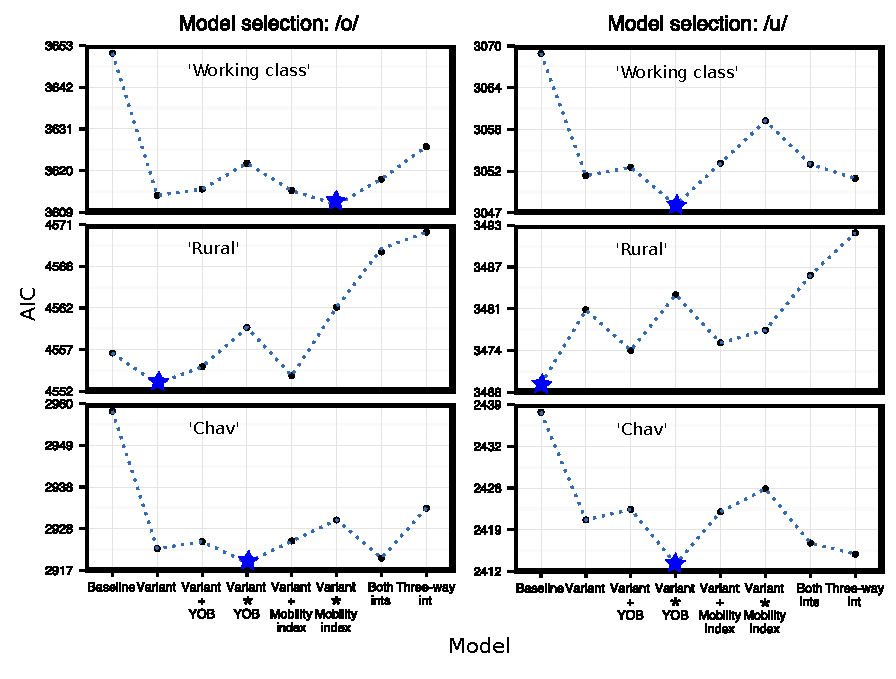
\includegraphics[scale=0.75]{model_comparison.pdf}
\end{figure}

 These models are compared in Figure 4 which plots the Akaike Information Criterion value for each model specification, arranged in order of model complexity. A lower AIC value indicates a better fit to the data. The best-fitting models are marked with a star. In terms of social class selections, the models for both /u/ and /o/ include the \textit{variant} term, confirming that listeners were able to use variation in these vowels as a reliable cue to socioeconomic status and to the \textsc{chav} subcategory. \textsc{rural}selections were reliably affected by variation in /o/, but not /u/. The best models for \textsc{working class} also include interaction terms for listener mobility (/o/) and year of birth (/u/), and the best models for \textsc{chav} include interaction terms for year of birth, indicating that listeners of different ages and social backgrounds behaved differently in the social perception task. Hypothesis tests were then conducted through a bootstrapped likelihood ratio test comparing models with and without each term (table x).

 \begin{table}[ht]
 \small
\centering
\begin{tabular}{llllllll}
  \hline
 /o/& Chisq & Df & P(ChiSq) & /u/&Chisq & Df & P(ChiSq) \\ 
  \hline
 \textbf{\textsc{working}}&&&  &\textbf{\textsc{working}}&&&\\ 
  \textbf{\textsc{class}}&&&  & \textbf{\textsc{class}}&&&\\
  \textit{Variant}& 51.64 & 7.00 & $<$0.0001 &  \textit{Variant}& 27.29 & 5.00 & $<$0.0001 \\  
  \textit{Variant*Mobility}& 18.42 & 8.00 & 0.02 &  \textit{Variant*Age}& 16.18 & 6.00 & 0.01 \\ 
\textbf{\textsc{rural}}&&&  & \textbf{\textsc{chav}}&&&\\ 
  \textit{Variant}& 17.37 & 7.00 & 0.01 &  \textit{Variant}& 27.74 & 5.00 & $<$0.0001 \\ 
\textbf{\textsc{chav}}&&& &  \textit{Variant*Age}& 19.25 & 6.00 & $<$0.01 \\ 
  \textit{Variant}& 49.39 & 7.00 & $<$0.0001&&&& \\ 
  \textit{Variant*Age}& 19.68 & 8.00 & 0.01&&&& \\
   \hline
\end{tabular}
\end{table}
\newpage
\subsection{Results: Main effects}
\subsubsection{/u/}
\begin{figure}[ht]
\centering
\caption{Main effects for /u/}
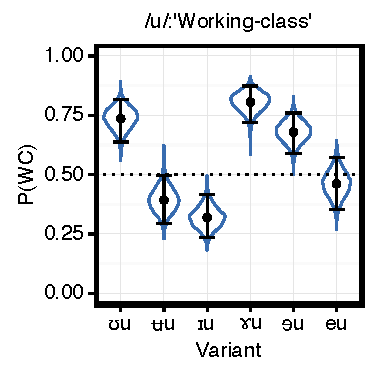
\includegraphics[scale=0.65]{uw_class.pdf}
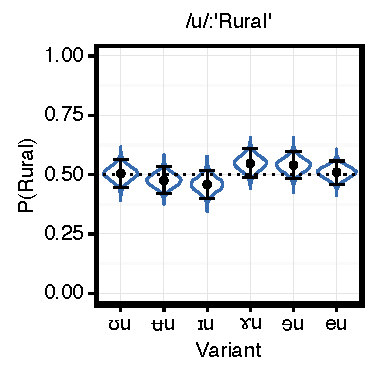
\includegraphics[scale=0.65]{uw_local.pdf}
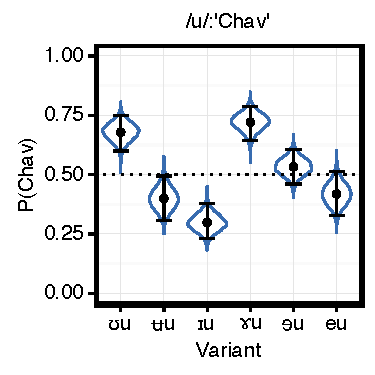
\includegraphics[scale=0.65]{uw_chav.pdf}
\end{figure}
Figure 5 demonstrates how variation in /u/ affected listeners selections in terms of the social categories \textsc{working class}, \textsc{rural} and \textsc{chav}. The points represent the mean predicted probability of each selection, with error bars showing the upper and lower bounds of the Highest Posterior Density interval, estimated through 10000 posterior samples. There is a clear effect of fronting on \textsc{working-class} selections, whereby fronter /u/ variants are more likely to cue middle-class selections and back variants are more likely to cue working-class selections. /u/ diphthongization seems to be weakly associated with \textsc{working class}, in that diphthongization weakens the effect of fronting (evident in the shallower slope of fronting across more diphthongal /u/ variants, and in the fact that the HPD interval for fronted, diphthongal /u/ crosses the p=.5 line. /u/ variants show no reliable effect on listeners' \textsc{rural} selections, while the results for \textsc{chav} mirror those for \textsc{working class}. 
These results contrast with the predictions formed earlier, where it was suggested that \textsc{/u/} variation would be perceived as relatively socially unmarked given its lack of social stratification in production. Despite the fact that /u/ fronting appears to have been adopted in a relatively uniform manner in this community, listeners consistently map innovative variants to the \textsc{middle class} category. 

\subsubsection{/o/}
\begin{figure}[ht]
\centering
\caption{Main effects for /o/}
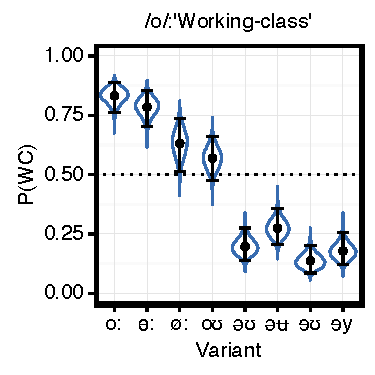
\includegraphics[scale=0.65]{ow_class.pdf}
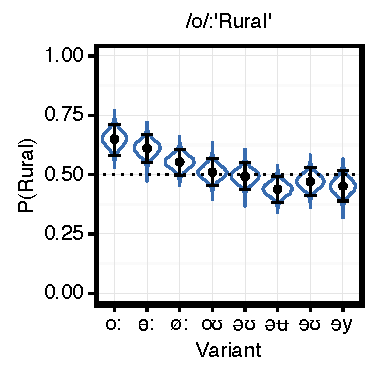
\includegraphics[scale=0.65]{ow_local.pdf}
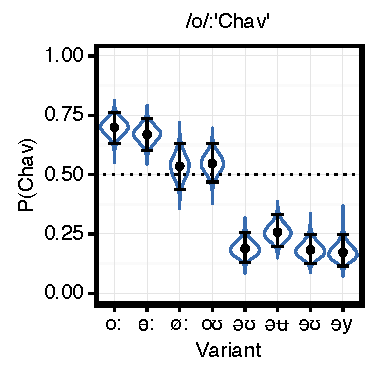
\includegraphics[scale=0.65]{ow_chav.pdf}
\end{figure}

Figure 6 visualizes the effect variant on social selections for /o/. In terms of \textsc{working class} selections, there is a clear effect of diphthongization, with more diphthongal variants reliably cueing the selection of a middle class image, and monophthongal variants cueing the selection of working-class image. The only exception to this pattern is back, diphthongal /o/; the fact that the interval for this variant crosses zero means that we cannot be certain that it had a reliable effect in either direction, but the fact that the interval is biased above the p=.5 line suggests that listeners tended to select working-class images when hearing this variant. Monophthongs all reliably predict the selection of a working-class image, but the strength of this effect weakens for more fronted variants. Note that this weakening effect of fronting holds for both diphthongs and monophthongs, in contrast to what might be predicted based on Haddican et al. (2013). 

In terms of \textsc{rural} selections, /o/ shows a weak but reliable effect for monophthongal variants. While diphthongs all show no reliable effect (in that the HPD interval crosses p=.5), monophthongs reliably cue the selection of a rural character. The fact that only monophthongs show reliable effects suggests that while /o/ monophthongs are associated with rural speech, the converse is not true of diphthongs. Overall, the results are broadly consistent with our earlier predictions -- listeners reliably map /o/ monophthongs to the \textsc{rural} category.

A key prediction based on Haddican et al.'s (2013) proposal was that fronted /o/ monophthongs would be associated with the \textsc{chav} subcategory. The data for /o/ provide no support for this proposal -- rather, \textsc{chav} selections mirror the effects for general  \textsc{working class} selections. While the most back /o/ variants reliably cue \textsc{chav} selections, fronted /o/ shows no reliable effect, and the overall trend is for fronting to \textit{lower} the probablity of a \textsc{chav} selection -- the opposite to what would be expected under the Haddican et al. (2013) account.



\subsection{Results: Listener variation}
A further prediction made in section 3.1.4 was that listeners would vary in their social perception of variation in /o/ and /u/. In particular, it was predicted that the \textsc{chav} association between fronted /o/ monophthongs and back /o/ diphthongs would be strongest among younger listeners. While no evidence was found for the predicted relationship between /o/ variation and \textsc{chav}, the data still provide evidence of variation in social perception, demonstrated below.
\subsubsection{\textsc{working class} selections}
\begin{figure}[ht]
\centering
\caption{Interaction effects: \textsc{working class} selections}
\subfigure[]{
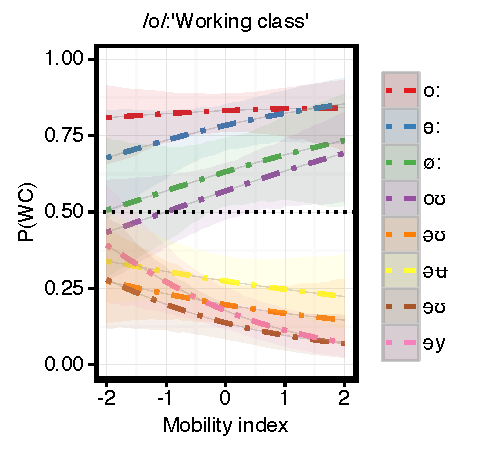
\includegraphics[scale=0.6]{ow_class_dim3.pdf}
}
\subfigure[]{
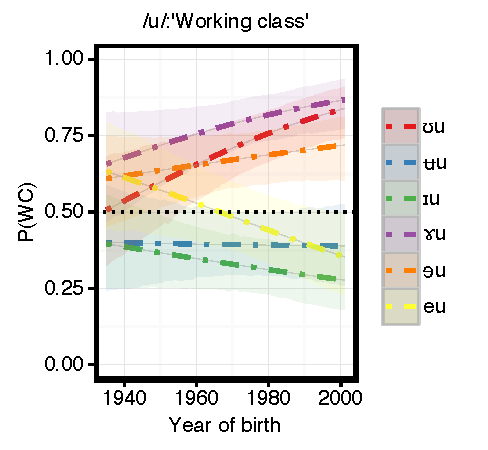
\includegraphics[scale=0.6]{uw_class_age.pdf}
}
\end{figure}
Figure 7 demonstrates variation in social class selections as a function of listener year of birth and the mobility index. For /o/, there is a significant effect of listener mobility (7a), with more mobile listeners generally more sensitive to the monophthong-diphthong distinction as a cue to socioeconomic status. The largest variation appears to be in the perception of the most fronted diphthong and most back monophthong -- these variants have a limited effect on the responses of less mobile listeners, suggesting that those listeners hear them as comparatively unmarked. In contrast, more mobile listeners tend to associated these variants with middle-class characters. /u/ selections show no evidence of variation in terms of mobility, but a significant effect of listener age (7b). Older listeners are generally less sensitive to fronting as a cue to socioeconomic status.
\subsubsection{\textsc{chav} selections}
\begin{figure}[ht]
\centering
\caption{Interaction effects: \textsc{chav} selections}
\subfigure[]{
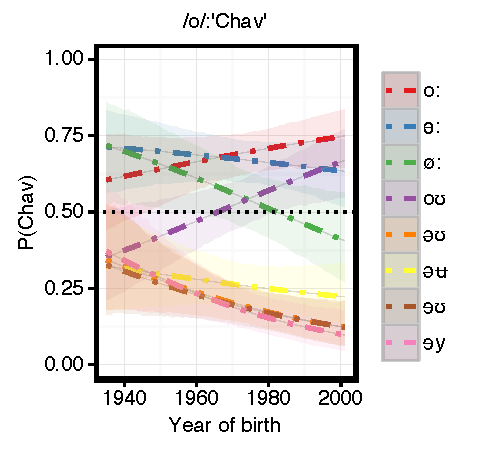
\includegraphics[scale=0.6]{ow_chav_age.pdf}}
\subfigure[]{
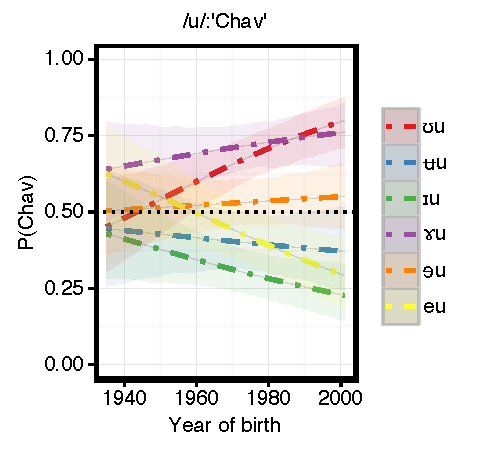
\includegraphics[scale=0.6]{uw_chav_age.pdf}}
\end{figure}
Figure 8 demonstrates the interaction of listener year of birth and variant heard on \textsc{chav} selections. In the case of /o/ (8a), it appears that younger listeners are more sensitive to diphthongs as an index of `non-Chav', whilst back, diphthongal and fronted, monophthongal /o/ show an interesting `cross-over' pattern: for older speakers, \textipa{[oU]} weakly disfavours \textsc{chav} selections, while for younger speakers it is reliably associated with \textsc{chav}; while [o:] reliably cues a \textsc{chav} selection for older listeners, it weakly disfavours such selections among younger listeners. For /u/ (8b), the effect of age is similar to that for \textsc{working-class} selections -- younger listeners map the back-front dimension of /u/ more reliably to the \textsc{chav} character than older listeners. 
\section{Conclusion}

\bibliographystyle{pwpl.bst}
\nocite{*}
\bibliography{reviewbib_short.bib}
\end{document}